\begin{figure}[tb]
\centering
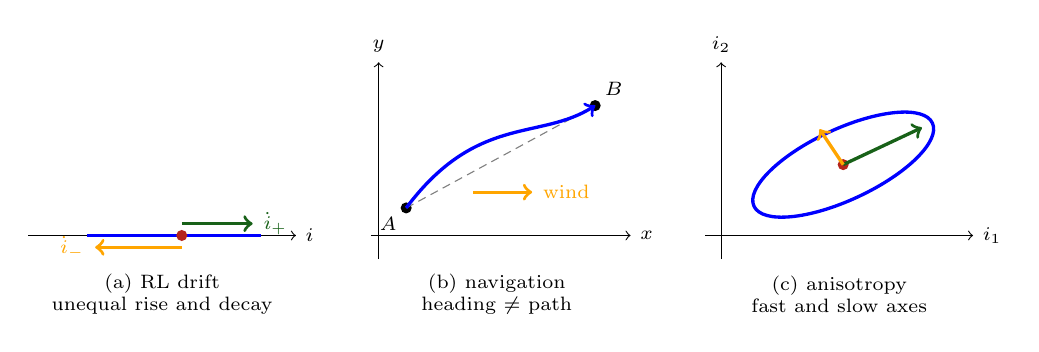
\begin{tikzpicture}[x=1cm,y=1cm,font=\scriptsize]
  \begin{scope}[shift={(0,0)}]
    \draw[->] (-.2,0)--(3.2,0) node[right] {$i$};
    \draw[very thick,blue] (.55,0)--(2.75,0);
    \fill[BrickRed] (1.75,0) circle (2pt);
    \draw[->,ForestGreen!70!black,very thick] (1.75,.15)--(2.65,.15) node[right] {$\dot i_+$};
    \draw[->,Orange,very thick] (1.75,-.15)--(.65,-.15) node[left] {$\dot i_-$};
    \node[align=center] at (1.5,-.75) {(a) RL drift\\unequal rise and decay};
  \end{scope}
  \begin{scope}[shift={(4.25,0)}]
    \draw[->] (-.1,0)--(3.2,0) node[right] {$x$};
    \draw[->] (0,-.3)--(0,2.2) node[above] {$y$};
    \fill (0.35,.35) circle (2pt) node[below left] {$A$};
    \fill (2.75,1.65) circle (2pt) node[above right] {$B$};
    \draw[densely dashed,gray] (.35,.35)--(2.75,1.65);
    \draw[blue,very thick,->] (.35,.35)..controls(1.25,1.55)and(2.05,1.2)..(2.75,1.65);
    \draw[->,Orange,very thick] (1.2,.55)--(1.95,.55) node[right] {wind};
    \node[align=center] at (1.5,-.75) {(b) navigation\\heading $\neq$ path};
  \end{scope}
  \begin{scope}[shift={(8.6,0)}]
    \draw[->] (-.2,0)--(3.2,0) node[right] {$i_1$};
    \draw[->] (0,-.3)--(0,2.2) node[above] {$i_2$};
    \draw[blue,very thick,rotate around={25:(1.55,.9)}] (1.55,.9) ellipse (1.25 and .45);
    \fill[BrickRed] (1.55,.9) circle (2pt);
    \draw[->,ForestGreen!70!black,very thick] (1.55,.9)--(2.55,1.37);
    \draw[->,Orange,very thick] (1.55,.9)--(1.25,1.35);
    \node[align=center] at (1.5,-.75) {(c) anisotropy\\fast and slow axes};
  \end{scope}
\end{tikzpicture}
\caption{Three concrete reasons why Euclidean current interpolation is not a
dynamic optimum: drift, advection, and anisotropic voltage-to-current speed.}
\label{fig:dynamic-primer}
\end{figure}

